%\documentclass[12pt,a4paper]{article}

\usepackage{graphicx}
\usepackage{bm}
\usepackage[utf8]{inputenc}
% caracteres utf8 (tildes, enie) sin tener que usar comandos

\usepackage{pdfpages} 
%para agregar pdfs(Karnaugh)

\usepackage[spanish, es-tabla, es-nodecimaldot]{babel}
% texto automatico en espaniol
% "tabla" en vez de "cuadro"
% no reemplaza puntos decimales por comas

%%%%%%%%%%%%%%%%%%%%%%%%%%%%%%%%%
%%%%%%%% PAQUETES EXTRA %%%%%%%%%
%%%%%%%%%%%%%%%%%%%%%%%%%%%%%%%%%

%Defino el papel y caracteristicas del informe
\usepackage[a4paper, total={6in, 8in}]{geometry}
\setlength{\parindent}{10pt}			%cuanta sangria al principio de un parrafo
\usepackage{indentfirst}				%pone sangria al primer parrafo de una seccion
\usepackage{graphicx} % importar imagenes
\usepackage{float} % posicion H para floats
\usepackage[colorinlistoftodos]{todonotes}
%Para realizar los mapas de Karnaugh (Sacado de https://tex.stackexchange.com/questions/140567/drawing-karnaughs-maps-in-latex)
%Macro para tablas de Karnaugh 
\usepackage{tikz}
\usetikzlibrary{matrix,calc}

%isolated term
%#1 - Optional. Space between node and grouping line. Default=0
%#2 - node
%#3 - filling color
\newcommand{\implicantsol}[3][0]{
    \draw[rounded corners=3pt, fill=#3, opacity=0.3] ($(#2.north west)+(135:#1)$) rectangle ($(#2.south east)+(-45:#1)$);}

%internal group
%#1 - Optional. Space between node and grouping line. Default=0
%#2 - top left node
%#3 - bottom right node
%#4 - filling color
\newcommand{\implicant}[4][0]{
    \draw[rounded corners=3pt, fill=#4, opacity=0.3] ($(#2.north west)+(135:#1)$) rectangle ($(#3.south east)+(-45:#1)$);
    }

%group lateral borders
%#1 - Optional. Space between node and grouping line. Default=0
%#2 - top left node
%#3 - bottom right node
%#4 - filling color
\newcommand{\implicantcostats}[4][0]{
    \draw[rounded corners=3pt, fill=#4, opacity=0.3] ($(rf.east |- #2.north)+(90:#1)$)-| ($(#2.east)+(0:#1)$) |- ($(rf.east |- #3.south)+(-90:#1)$);
    \draw[rounded corners=3pt, fill=#4, opacity=0.3] ($(cf.west |- #2.north)+(90:#1)$) -| ($(#3.west)+(180:#1)$) |- ($(cf.west |- #3.south)+(-90:#1)$);
}

%group top-bottom borders
%#1 - Optional. Space between node and grouping line. Default=0
%#2 - top left node
%#3 - bottom right node
%#4 - filling color
\newcommand{\implicantdaltbaix}[4][0]{
    \draw[rounded corners=3pt, fill=#4, opacity=0.3] ($(cf.south -| #2.west)+(180:#1)$) |- ($(#2.south)+(-90:#1)$) -| ($(cf.south -| #3.east)+(0:#1)$);
    \draw[rounded corners=3pt, fill=#4, opacity=0.3] ($(rf.north -| #2.west)+(180:#1)$) |- ($(#3.north)+(90:#1)$) -| ($(rf.north -| #3.east)+(0:#1)$);
}

%group corners
%#1 - Optional. Space between node and grouping line. Default=0
%#2 - filling color
\newcommand{\implicantcantons}[2][0]{
    \draw[rounded corners=3pt, opacity=.3] ($(rf.east |- 0.south)+(-90:#1)$) -| ($(0.east |- cf.south)+(0:#1)$);
    \draw[rounded corners=3pt, opacity=.3] ($(rf.east |- 8.north)+(90:#1)$) -| ($(8.east |- rf.north)+(0:#1)$);
    \draw[rounded corners=3pt, opacity=.3] ($(cf.west |- 2.south)+(-90:#1)$) -| ($(2.west |- cf.south)+(180:#1)$);
    \draw[rounded corners=3pt, opacity=.3] ($(cf.west |- 10.north)+(90:#1)$) -| ($(10.west |- rf.north)+(180:#1)$);
    \fill[rounded corners=3pt, fill=#2, opacity=.3] ($(rf.east |- 0.south)+(-90:#1)$) -|  ($(0.east |- cf.south)+(0:#1)$) [sharp corners] ($(rf.east |- 0.south)+(-90:#1)$) |-  ($(0.east |- cf.south)+(0:#1)$) ;
    \fill[rounded corners=3pt, fill=#2, opacity=.3] ($(rf.east |- 8.north)+(90:#1)$) -| ($(8.east |- rf.north)+(0:#1)$) [sharp corners] ($(rf.east |- 8.north)+(90:#1)$) |- ($(8.east |- rf.north)+(0:#1)$) ;
    \fill[rounded corners=3pt, fill=#2, opacity=.3] ($(cf.west |- 2.south)+(-90:#1)$) -| ($(2.west |- cf.south)+(180:#1)$) [sharp corners]($(cf.west |- 2.south)+(-90:#1)$) |- ($(2.west |- cf.south)+(180:#1)$) ;
    \fill[rounded corners=3pt, fill=#2, opacity=.3] ($(cf.west |- 10.north)+(90:#1)$) -| ($(10.west |- rf.north)+(180:#1)$) [sharp corners] ($(cf.west |- 10.north)+(90:#1)$) |- ($(10.west |- rf.north)+(180:#1)$) ;
}

%Empty Karnaugh map 4x4
\newenvironment{Karnaugh}%
{
\begin{tikzpicture}[baseline=(current bounding box.north),scale=0.8]
\draw (0,0) grid (4,4);
\draw (0,4) -- node [pos=0.7,above right,anchor=south west] {$X_1X_2$} node [pos=0.7,below left,anchor=north east] {$X_3X_4$} ++(135:1);
%
\matrix (mapa) [matrix of nodes,
        column sep={0.8cm,between origins},
        row sep={0.8cm,between origins},
        every node/.style={minimum size=0.3mm},
        anchor=8.center,
        ampersand replacement=\&] at (0.5,0.5)
{
                       \& |(c00)| 00         \& |(c01)| 01         \& |(c11)| 11         \& |(c10)| 10         \& |(cf)| \phantom{00} \\
|(r00)| 00             \& |(0)|  \phantom{0} \& |(1)|  \phantom{0} \& |(3)|  \phantom{0} \& |(2)|  \phantom{0} \&                     \\
|(r01)| 01             \& |(4)|  \phantom{0} \& |(5)|  \phantom{0} \& |(7)|  \phantom{0} \& |(6)|  \phantom{0} \&                     \\
|(r11)| 11             \& |(12)| \phantom{0} \& |(13)| \phantom{0} \& |(15)| \phantom{0} \& |(14)| \phantom{0} \&                     \\
|(r10)| 10             \& |(8)|  \phantom{0} \& |(9)|  \phantom{0} \& |(11)| \phantom{0} \& |(10)| \phantom{0} \&                     \\
|(rf) | \phantom{00}   \&                    \&                    \&                    \&                    \&                     \\
};
}%
{
\end{tikzpicture}
}

%Empty Karnaugh map 2x4
\newenvironment{Karnaughvuit}%
{
\begin{tikzpicture}[baseline=(current bounding box.north),scale=0.8]
\draw (0,0) grid (4,2);
\draw (0,2) -- node [pos=0.7,above right,anchor=south west] {$X_1X_2$} node [pos=0.7,below left,anchor=north east] {$X_3$} ++(135:1);
%
\matrix (mapa) [matrix of nodes,
        column sep={0.8cm,between origins},
        row sep={0.8cm,between origins},
        every node/.style={minimum size=0.3mm},
        anchor=4.center,
        ampersand replacement=\&] at (0.5,0.5)
{
                      \& |(c00)| 00         \& |(c01)| 01         \& |(c11)| 11         \& |(c10)| 10         \& |(cf)| \phantom{00} \\
|(r00)| 0             \& |(0)|  \phantom{0} \& |(1)|  \phantom{0} \& |(3)|  \phantom{0} \& |(2)|  \phantom{0} \&                     \\
|(r01)| 1             \& |(4)|  \phantom{0} \& |(5)|  \phantom{0} \& |(7)|  \phantom{0} \& |(6)|  \phantom{0} \&                     \\
|(rf) | \phantom{00}  \&                    \&                    \&                    \&                    \&                     \\
};
}%
{
\end{tikzpicture}
}

%Empty Karnaugh map 2x2
\newenvironment{Karnaughquatre}%
{
\begin{tikzpicture}[baseline=(current bounding box.north),scale=0.8]
\draw (0,0) grid (2,2);
\draw (0,2) -- node [pos=0.7,above right,anchor=south west] {$X_1$} node [pos=0.7,below left,anchor=north east] {$X_2$} ++(135:1);
%
\matrix (mapa) [matrix of nodes,
        column sep={0.8cm,between origins},
        row sep={0.8cm,between origins},
        every node/.style={minimum size=0.3mm},
        anchor=2.center,
        ampersand replacement=\&] at (0.5,0.5)
{
          \& |(c00)| 0          \& |(c01)| 1  \\
|(r00)| 0 \& |(0)|  \phantom{0} \& |(1)|  \phantom{0} \\
|(r01)| 1 \& |(2)|  \phantom{0} \& |(3)|  \phantom{0} \\
};
}%
{
\end{tikzpicture}
}

%Defines 8 or 16 values (0,1,X)
\newcommand{\contingut}[1]{%
\foreach \x [count=\xi from 0]  in {#1}
     \path (\xi) node {\x};
}

%Places 1 in listed positions
\newcommand{\minterms}[1]{%
    \foreach \x in {#1}
        \path (\x) node {1};
}

%Places 0 in listed positions
\newcommand{\maxterms}[1]{%
    \foreach \x in {#1}
        \path (\x) node {0};
}

%Places X in listed positions
\newcommand{\indeterminats}[1]{%
    \foreach \x in {#1}
        \path (\x) node {X};
}

%
%\begin{document}


\section{Algebra booleana y compuertas lógicas}

En el álgebra booleana se conoce como término canónico de una función lógica a todo producto o suma en la cual aparecen todas las variables en su forma directa o inversa. Cualquier función lógica puede expresarse de forma canónica utilizando los conceptos de min y maxtérminos. El primero, se refiere a todas las filas para las cuales la función lógica es igual a uno en la tabla de verdad correspondiente, mientras que el segundo se corresponde con todos los valores para los cuales la función es igual a cero. 

En el siguiente ejercicio se simplificarán dos funciones lógicas aplicando ambos conceptos. Luego se utilizarán mapas de Karnaugh para llegar a la misma expresión. A continuación se dibujará el circuito lógico resultante utilizando compuertas AND, OR y NOT, y por último, se usarán compuertas NAND exclusivamente.

\subsection{Primera Expresión: suma de productos}

\subsubsection{Simplificación mediante álgebra booleana}

La expresión de la cual se parte está dada por la siguiente fórmula:

\begin{equation}\label{eq:suma_minterminos}
f(e,d,c,b,a) = \sum{m(0, 2, 4, 7, 8, 10, 12, 16, 18, 20, 23, 24, 25, 26, 27, 28)}
\end{equation}

La ecuación \ref{eq:suma_minterminos} nos indica cuales entradas en la tabla de verdad son iguales a uno. A partir de ella podemos plantear la siguiente ecuación, la cual se trabajará para llegar a su respectiva expresión canónica.

\begin{multline}
\bar{e} \cdot \bar{d} \cdot \bar{c} \cdot \bar{b} \cdot \bar{a} + 
\bar{e} \cdot \bar{d} \cdot \bar{c} \cdot b \cdot \bar{a} +
\bar{e} 	\cdot \bar{d} \cdot c \cdot \bar{b} \cdot \bar{a} +
\bar{e} \cdot \bar{d} \cdot c \cdot b \cdot a + 
\bar{e} \cdot d \cdot \bar{c} \cdot \bar{b} \cdot \bar{a} + 
\bar{e} \cdot d \cdot \bar{c} \cdot b \cdot \bar{a} + 
\bar{e} \cdot d \cdot c \cdot \bar{b} \cdot \bar{a} + 
e \cdot \bar{d} \cdot \bar{c} \cdot \bar{b} \cdot \bar{a} + \\
e \cdot \bar{d} \cdot \bar{c} \cdot b \cdot \bar{a} + 
e \cdot \bar{d} \cdot c \cdot \bar{b} \cdot \bar{a} + 		
e \cdot \bar{d} \cdot c \cdot b \cdot a + 
e \cdot d \cdot \bar{c} \cdot \bar{b} \cdot \bar{a} + 
e \cdot d \cdot \bar{c} \cdot \bar{b} \cdot a + 
e \cdot d \cdot \bar{c} \cdot b \cdot \bar{a} + 
e \cdot d \cdot \bar{c} \cdot b \cdot a +
e \cdot d \cdot c \cdot \bar{b} \cdot \bar{a} 
\end{multline}

La expresión anterior puede parecer complicada en un principio, pero esta ordenada según cada mintermino correspondiente. Para comenzar el proceso de simplificación, gracias a la ley de idempotencia se puede sumar términos ya presentes en la ecuación anterior. So procederá a duplicar los mintérminos 2, 18 y 26 y a ordenar la fórmula para facilitar la simplificación. 

\begin{equation}
\bar{e} \cdot \bar{d} \cdot \bar{c} \cdot \bar{b} \cdot \bar{a} +  %0
\bar{e} \cdot \bar{d} \cdot \bar{c} \cdot b \cdot \bar{a} +        %2
e \cdot \bar{d} \cdot \bar{c} \cdot \bar{b} \cdot \bar{a} +    	  %16
e \cdot \bar{d} \cdot \bar{c} \cdot b \cdot \bar{a}  	          %18
\end{equation}

\begin{equation}
\bar{e} \cdot d \cdot \bar{c} \cdot b \cdot \bar{a} + 		      %10
e \cdot d \cdot \bar{c} \cdot b \cdot \bar{a} + 	                  %26
\bar{e} \cdot \bar{d} \cdot \bar{c} \cdot b \cdot \bar{a} +        %2
e \cdot \bar{d} \cdot \bar{c} \cdot b \cdot \bar{a}  	          %18
\end{equation}

\begin{equation}
\bar{e} 	\cdot \bar{d} \cdot c \cdot \bar{b} \cdot \bar{a} +	      %4
\bar{e} \cdot d \cdot c \cdot \bar{b} \cdot \bar{a} + 			  %12
e \cdot \bar{d} \cdot c \cdot \bar{b} \cdot \bar{a} + 		      %20
e \cdot d \cdot c \cdot \bar{b} \cdot \bar{a}                      %28
\end{equation}

\begin{equation}
e \cdot d \cdot \bar{c} \cdot \bar{b} \cdot \bar{a} +              %24
e \cdot d \cdot \bar{c} \cdot \bar{b} \cdot a +                    %25
e \cdot d \cdot \bar{c} \cdot b \cdot \bar{a} + 	                  %26
e \cdot d \cdot \bar{c} \cdot b \cdot a                           %27
\end{equation}

\begin{equation}
e \cdot \bar{d} \cdot c \cdot b \cdot a +                          %23
\bar{e} \cdot \bar{d} \cdot c \cdot b \cdot a  			          %7
\end{equation}

Las sumas de productos anteriores pueden trabajarse si se factorizan por los términos apropiados:

\begin{equation}\label{eq:minterm_0_2_16_18}
\bar{d} \cdot \bar{c} \cdot \bar{a} \cdot (\bar{e} \cdot \bar{b} + \bar{e} \cdot b + e \cdot \bar{b} + e \cdot b)
\end{equation}

\begin{equation}\label{eq:mintem_10_26_2_18}
\bar{c} \cdot b \cdot \bar{a} \cdot (\bar{e} \cdot b + e 	\cdot d + \bar{e} \cdot \bar{d} + e \cdot \bar{d})
\end{equation}

\begin{equation}\label{eq:minterm_4_12_20_28}
c \cdot \bar{b} \cdot \bar{a} \cdot (\bar{e} \cdot \bar{d} + \bar{e} \cdot d + e \cdot \bar{d} + e \cdot d)
\end{equation}

\begin{equation}\label{eq:minterm_24_25_26_27}
e \cdot d \cdot c \cdot (\bar{b} \cdot \bar{a} + \bar{b} \cdot a + b \cdot \bar{a} + b \cdot a)
\end{equation}

\begin{equation}\label{eq:minterm_/_23}
\bar{d} \cdot c \cdot b \cdot a \cdot (\bar{e} + e)
\end{equation}

Luego aplicando la propiedad de combinación en todos los productos:

\begin{equation}\label{eq:minterm_0_2_16_18}
\bar{d} \cdot \bar{c} \cdot \bar{a} \cdot (\bar{e} \cdot \bar{b} + \bar{e} \cdot b + e \cdot \bar{b} + e \cdot b)
\end{equation}

\begin{equation}\label{eq:mintem_10_26_2_18}
\bar{c} \cdot b \cdot \bar{a} \cdot (\bar{e} \cdot b + e 	\cdot d + \bar{e} \cdot \bar{d} + e \cdot \bar{d})
\end{equation}

\begin{equation}\label{eq:minterm_4_12_20_28}
c \cdot \bar{b} \cdot \bar{a} \cdot (\bar{e} \cdot \bar{d} + \bar{e} \cdot d + e \cdot \bar{d} + e \cdot d)
\end{equation}

\begin{equation}\label{eq:minterm_24_25_26_27}
e \cdot d \cdot c \cdot (\bar{b} \cdot \bar{a} + \bar{b} \cdot a + b \cdot \bar{a} + b \cdot a)
\end{equation}

\begin{equation}\label{eq:minterm_7_23}
\bar{d} \cdot c \cdot b \cdot a \cdot (\bar{e} + e)
\end{equation}


En \ref{eq:minterm_0_2_16_18}, \ref{eq:mintem_10_26_2_18}, \ref{eq:minterm_4_12_20_28} y \ref{eq:minterm_24_25_26_27} se puede aplicar la propiedad de combinación, mientras que en \ref{eq:minterm_/_23} se utiliza la ley del complemento:

\begin{equation}\label{eq:minterm_0_2_16_18_Simp}
\bar{d} \cdot \bar{c} \cdot \bar{a} \cdot (\bar{e} + e)
\end{equation}

\begin{equation}\label{eq:mintem_10_26_2_18_Simp}
\bar{c} \cdot b \cdot \bar{a} \cdot (d + \bar{d})
\end{equation}

\begin{equation}\label{eq:minterm_4_12_20_28_Simp}
c \cdot \bar{b} \cdot \bar{a} \cdot (\bar{e} + e)
\end{equation}

\begin{equation}\label{eq:minterm_24_25_26_27_Simp}
e \cdot d \cdot c \cdot (\bar{b} + b)
\end{equation}

\begin{equation}\label{eq:minterm_7_23_Simp}
\bar{d} \cdot c \cdot b \cdot a 
\end{equation}

Sumando \ref{eq:minterm_0_2_16_18_Simp}, \ref{eq:mintem_10_26_2_18_Simp}, \ref{eq:minterm_4_12_20_28_Simp}, \ref{eq:minterm_24_25_26_27_Simp} y \ref{eq:minterm_7_23_Simp}:

\begin{equation}
\bar{d} \cdot \bar{c} \cdot \bar{a} \cdot (\bar{e} + e) + 
\bar{c} \cdot b \cdot \bar{a} \cdot (d + \bar{d}) + 
c \cdot \bar{b} \cdot \bar{a} \cdot (\bar{e} + e) + 
e \cdot d \cdot c \cdot (\bar{b} + b) +
\bar{d} \cdot c \cdot b \cdot a 
\end{equation}

Finalmente se aplica nuevamente la ley del complemento en los cuatro primeros productos y se llega a la expresión final:

\begin{equation}\label{canonica_minterm}
\boxed{\bar{d} \cdot \bar{c} \cdot \bar{a} + 
\bar{c} \cdot b \cdot \bar{a} + 
c \cdot \bar{b} \cdot \bar{a} + 
e \cdot d \cdot c \cdot + 
\bar{d} \cdot c \cdot b \cdot a}
\end{equation}


\subsubsection{Simplificación mediante mapas de Karnaugh}

Otro método oara conseguir la mínima expresión posible es mediante mapas de Karnaugh. A continaución se utilizó un mapa de Karnaugh de 5 variables con el fin de llegar a la expresión canónica:
\begin{figure}[H]
   \centering
\begin{tabular}{ccc}
	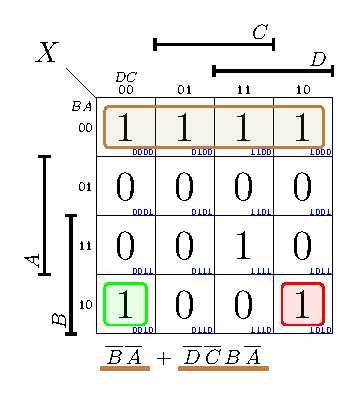
\includegraphics[width=4cm,trim={0.25cm 0.5cm  0.25cm 0.25cm},clip]{Ejercicio_2/Karnaugh/K1.pdf}& \hspace{3ex} 
	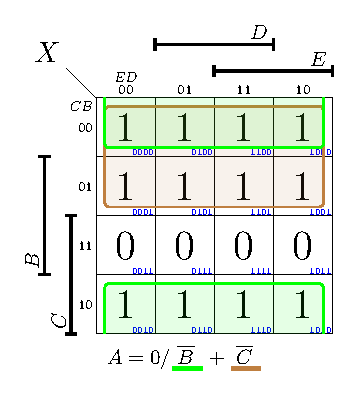
\includegraphics[width=4cm,trim={0.25cm 0.5cm  0.25cm 0.25cm},clip]{Ejercicio_2/Karnaugh/K2.pdf}&
	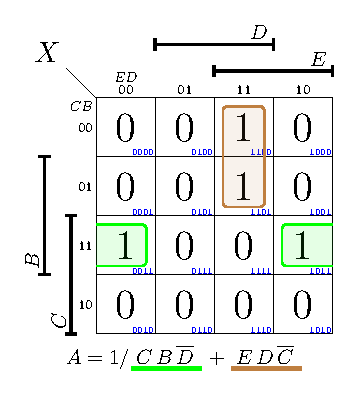
\includegraphics[width=4cm,trim={0.25cm 0.5cm  0.25cm 0.25cm},clip]{Ejercicio_2/Karnaugh/K3.pdf}\\
	\end{tabular}
    \label{fig:Karnaughs_encoder} % 
\end{figure}

 


    \begin{table}[H]
        \begin{center}
            \def\arraystretch{1.5}
            \begin{tabular}{|c|c|}
                \hline
                (0,2,8,10,16,18,24,26) &	$\bar{C}\bar{E}$ \\
                \hline
                (0,4,8,12,16,20,24,28) & $\bar{D}\bar{E}$ \\
                \hline  
                (24,25,26,27) & $AB\bar{C}$ \\
                \hline   
                (7,23) & $\bar{B}CDE$ \\
                \hline           
                
            \end{tabular}
            %\caption{Tabla de verdad del Demultiplexor}
        \end{center}

    \end{table}


    
    \begin{table}[H]
        \begin{center}
            \def\arraystretch{1.5}
            \begin{tabular}{|c|c|c|c|c|}
                \hline
                &	$\bar{D}\bar{E}$ &	$\bar{D}E$ &	$D\bar{E}$ & $DE$ \\
                \hline
                $\bar{A}\bar{B}\bar{C}$ & 1 & 0 & 0 & 1 \\
                \hline          
                $\bar{A}\bar{B}C$ & 1 & 0 & 1 & 0 \\
                \hline   
                $\bar{A}BC$ & 1 & 0 & 0 & 0 \\
                \hline     
                $\bar{A}B\bar{C}$  & 1 & 0 & 0 & 1 \\
                \hline
                
                $A\bar{B}\bar{C}$ & 1 & 0 & 0 & 1 \\
                
                \hline
                
                $A\bar{B}C$ & 1 & 0 & 1 & 0 \\
                \hline
                
                $ABC$ & 1 & 0 & 0 & 0 \\
                \hline
                
                $AB\bar{C}$ & 1 & 1 & 1 & 1 \\
                \hline
                
            \end{tabular}
            %\caption{Tabla de verdad del Demultiplexor}
        \end{center}

    \end{table}



    \begin{table}[H]
        \begin{center}
            \def\arraystretch{1.5}
            \begin{tabular}{|c|c|c|c|c|}
                \hline
                &	$\bar{D}\bar{E}$ &	$\bar{D}E$ &	$D\bar{E}$ & $DE$ \\
                \hline
                $\bar{A}\bar{B}\bar{C}$ & 0 & 1 & 3 & 2 \\
                \hline          
                $\bar{A}\bar{B}C$ & 4 & 5 & 7 & 6 \\
                \hline   
                $\bar{A}BC$ & 12 & 13 & 15 & 14 \\
                \hline     
                $\bar{A}B\bar{C}$  & 8 & 9 & 11 & 10 \\
                \hline
                
                $A\bar{B}\bar{C}$ & 16 & 17 & 19 & 18 \\
                
                \hline
                
                $A\bar{B}C$ & 20 & 21 & 23 & 22 \\
                \hline
                
                $ABC$ & 28 & 29 & 31 & 30 \\
                \hline
                
                $AB\bar{C}$ & 24 & 25 & 27 & 26 \\
                \hline
                
            \end{tabular}
            %\caption{Tabla de verdad del Demultiplexor}
        \end{center}

    \end{table}


\subsubsection{Implementación mediante compuertas AND, OR y NOT}

La expresión obtenida en \ref{canonica_minterm} puede ser implementada mediante compuertas lógicas facilmente:


\begin{figure}[H]
\centering
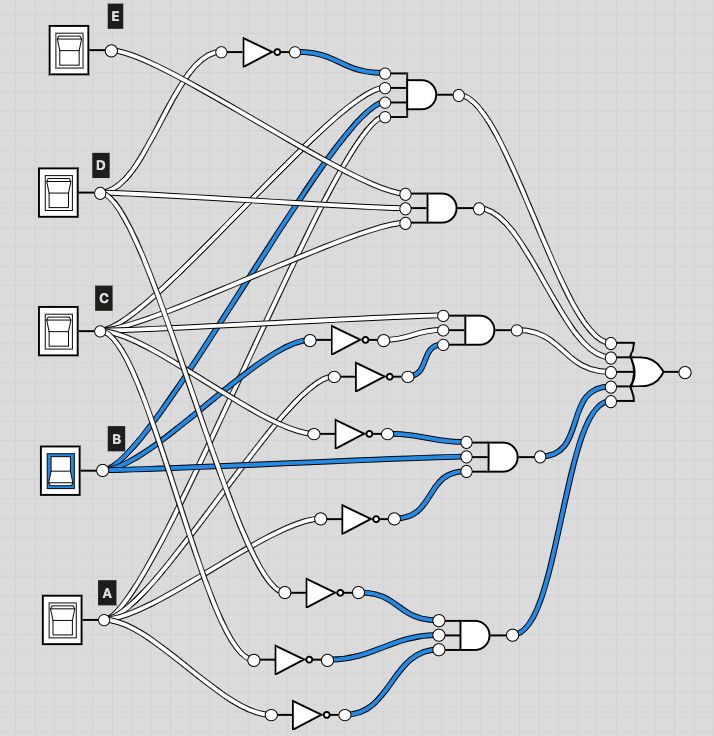
\includegraphics[width=12cm,height=8cm]{Ejercicio_2/circuitos/Ej2_parte1_logicly.png}
\end{figure}

\subsubsection{Implementación mediante compuertas NAND}
A su vez el circuito anterior implementado mediante compuertas nand queda de la siguiente manera:

\begin{figure}[H]
\centering
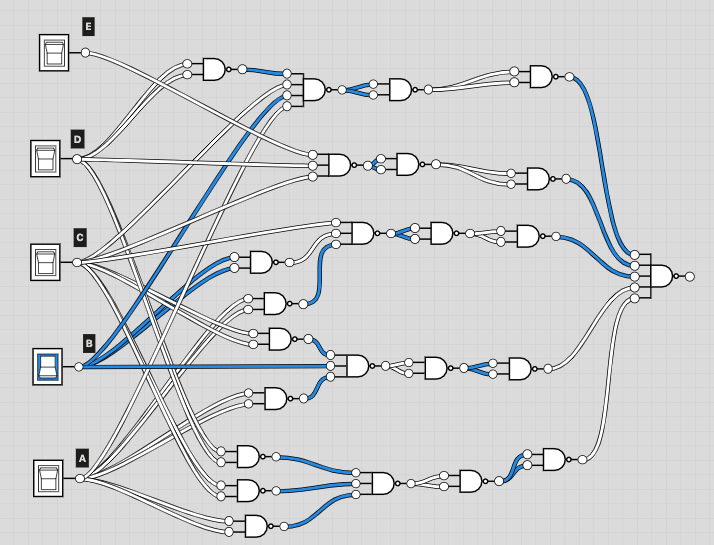
\includegraphics[width=12cm,height=8cm]{Ejercicio_2/circuitos/Ej2_parte1_nand_logicly.png}
\end{figure}



\subsection{Segunda expresión: producto de sumas}
Por último, se sabe que tanto las compuertas AND, OR o NOT pueden ser representadas usando compuertas NAND unicamente. A continaución se realizó el mismo circuito lógico solo con compuertas NAND:


\subsubsection{Simplificación mediante álgebra booleana}
Para la segunda parte del ejercicio, se comienza a partir del siguiente producto de sumas:
\begin{equation}\label{eq:prod_maxterminos}
f(d,c,b,a) = \prod{M_0, M_2, M_4, M_7, M_8, M_10, M_12)}
\end{equation}

A a partir de \ref{eq:prod_maxterminos} se define la siguiente expresion:

\begin{equation}
(d + c + b +a) \cdot (d + c + \bar{b} + a) \cdot (d + \bar{c} +b +a) \cdot (d + \bar{c} + \bar{b} + \bar{a}) 	\cdot (\bar{d} + c + b + a) \cdot (\bar{d} + c + \bar{b} + a) \cdot (\bar{d} + \bar{c} + b + a)
\end{equation}

En este caso se usa nuevamente la propiedad de idempotencia, en este caso para un producto, para duplicar el mintermino número 8 y 0 y así facilitar el trabajo algebraico. Luego se separan los productos en tres grupos para su posterior factorización:

\begin{equation}\label{Maxterm_0_2_8_10}
(d + c + b +a) \cdot (d + c + \bar{b} + a) \cdot (\bar{d} + c + b + a) \cdot (\bar{d} + c + \bar{b} + a)
\end{equation}

\begin{equation}\label{Maxterm_0_4_8_12}
(d + c + b +a) \cdot (d + \bar{c} +b +a) \cdot (\bar{d} + c + b + a) \cdot (\bar{d} + \bar{c} + b + a)
\end{equation}

\begin{equation}\label{Maxterm_7}
(d + \bar{c} + \bar{b} + \bar{a})
\end{equation}

Tanto en \ref{Maxterm_0_2_8_10} como en \ref{Maxterm_0_4_8_12} es posible usar la propiedad de combianción para el producto entre los primeros dos y los últimos dos términos para simplificar las expresiones. \ref{Maxterm_7} esta expresado en forma canóncia.

\begin{equation}\label{Maxterm_0_2_8_10_simp}
(d + c + a) \cdot (\bar{d} + c + a) 
\end{equation}

\begin{equation}\label{Maxterm_0_4_8_12_simp}
(d + b +a) \cdot (\bar{d} + b + a)
\end{equation}

Luego se utiliza la propiedad de combianción para el producto nuevamente, en ambas ecuaciones:

\begin{equation}\label{Maxterm_0_2_8_10_final}
(c + a) 
\end{equation}

\begin{equation}\label{Maxterm_0_4_8_12_final}
(b +a)
\end{equation}

Por último se unen \ref{Maxterm_0_2_8_10_final}, \ref{Maxterm_0_4_8_12_final} y \ref{Maxterm_7} para llegar a una expresión final:

\begin{equation}\label{eq:max_final}
\boxed{(c + a) \cdot (b +a) \cdot (d + \bar{c} + \bar{b} + \bar{a})}
\end{equation}

\subsubsection{Simplificacioón mediante mapas de Karnaugh}
Al igual que en el punto anterior, se utilizaron mapas de KArnaugh para llegar a la mínima expresión posible:


\subsubsection{Implementación mediante compuertas AND, OR y NOT}

A continuación se implementó la función obtenida en \ref{eq:max_final} mediante compuertas AND, OR y NOT:

\begin{figure}[H]
\centering
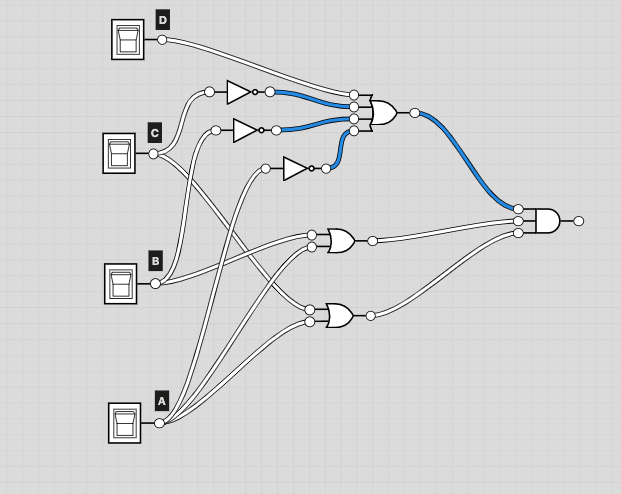
\includegraphics[width=10cm,height=6cm]{Ejercicio_2/circuitos/Ej2_parte2_logily.png}
\end{figure}

\subsubsection{Implementación mediante compuertas NAND}
Por último se realizó el circuito anterior solamente con compuertas NAND:
\begin{figure}[H]
\centering
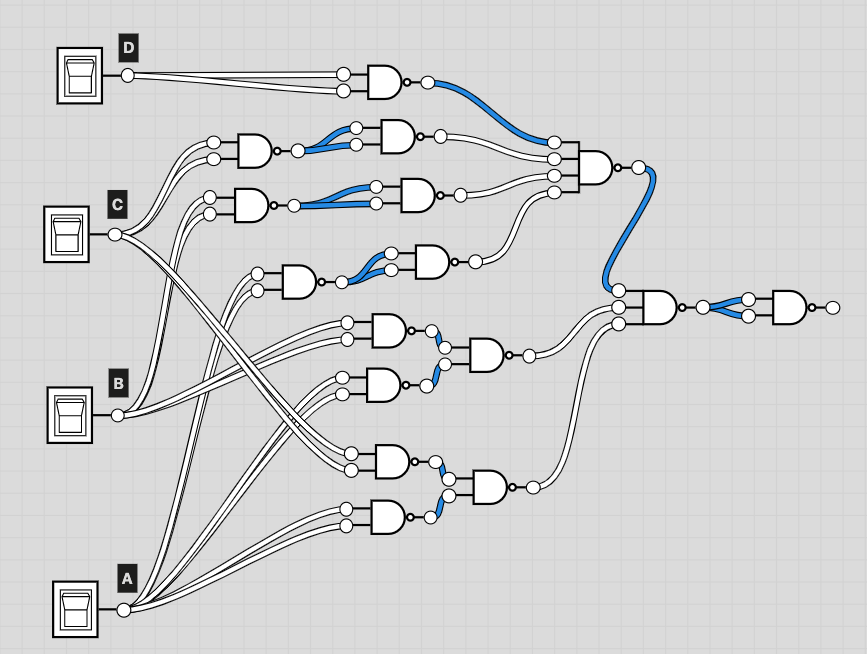
\includegraphics[width=10cm,height=6cm]{Ejercicio_2/circuitos/Ej2_parte2_nand_logicly.png}
\end{figure}

%\end{document}